\documentclass[11pt]{article}

\usepackage{amsmath}
\usepackage{graphicx}
\usepackage[width=288pt,justification=centering,aboveskip=18pt,belowskip=18pt]{caption}
\usepackage{mathrsfs}
\usepackage{pdflscape}
\usepackage{verbatim}

\title{System Planning Toolbox}
\author{Raymond A. LeClair}
\date{\today}

\begin{document}

\maketitle

\begin{abstract}
The System Planning Toolbox performs the engineering analysis required
for the coordination of communication networks under national and
international regulatory criteria with a focus on the
Radiocommunication Sector Space Services.  The toolbox is implemented
in MATLAB using an object-oriented approach, and calculates equivalent
power flux density (EPFD) up, down, and inter-satellite for comparison
with Article 22 limits.
\end{abstract}

\section{Introduction}

The System Planning Toolbox performs the engineering analysis required
for the coordination of communication networks under regulatory
criteria of the U.S. Federal Communications Commission (FCC) and the
International Telecommunications Union (ITU) with a focus on the
Radiocommunication Sector Space Services. The communication network,
or system, may consist of an arbitrary Earth and space segment, with
the space segment consisting of geostationary or non-geostationary
satellites. The toolbox:
\begin{itemize}
\item Implements Earth and space transmitting and receiving antenna
  patterns as defined in the ITU antenna pattern library
\item Models space station orbits as two-body orbits optionally
  including J2 effects
\item Models Earth station position using WGS84
\item Models multiple beams per space station, accounting for beam
  multiplexing, and implements simplified beam assignment algorithms
\item Calculates equivalent power flux density (EPFD) up, down, and
  inter-satellite
\end{itemize}

\section{Getting Started}

The System Planning Toolbox is implemented in MATLAB using an
object-oriented approach and consists of the packages and classes
shown in summary form in table \ref{table-packages-and-classes}. Note
that package names beginning with “+” follow the MATLAB convention for
name space creation. All classes have a corresponding test class, not
shown, which implement unit tests of public, and some private,
methods.

\begin{landscape}
  \begin{table}
    \caption{System Planning Toolbox Packages and Classes}\label{table-packages-and-classes}
\small
\begin{verbatim}
com                              com                                        com
|__ springbok                    |__ springbok                              |__ celestrak
    |__ antenna                      |__ simulation                         │   |__ sgp4v
    |   |__ Antenna.m                |   |__ +example                       |       |__ *.m (Functions)
    |   |__ EarthStationAntenna.m    |   |   |__ Plot.m                     |__ springbok
    |   |__ SpaceStationAntenna.m    |   |   |__ Simulate.m                 |   |__ operator
    |__ pattern                      |   |   |__ getIntLeoEarthSegment.m    |   |   |__ HohmannTransfer.m
    |   |__ EarthPattern.m           |   |   |__ getIntLeoSpaceSegment.m    |   |   |__ OrbitDetermination.m
    |   |__ Pattern.m                |   |   |__ getSystems.m               |   |   |__ SatelliteCatalog.m
    |   |__ PatternE*.m (Earth)      |   |   |__ getWntGsoEarthSegment.m    |   |   |__ SimulationConstants.m
    |   |__ PatternS*.m (Space)      |   |   |__ getWntGsoSpaceSegment.m    |   |__ sgp4v
    |   |__ ReceivePattern.m         |   |__ +spacex                        |       |__ Sgp4Coordinates.m
    |   |__ SpacePattern.m           |       |__ Plot.m                     |       |__ Sgp4Orbit.m
    |   |__ TransmitPattern.m        |       |__ Simulate.m                 |       |__ Sgp4OrbitTest.m
    |__ station                      |       |__ getEdges.m                 |__ utility                              
    |   |__ Beam.m                   |       |__ getIntLeoEarthSegment.m        |__ Article22Utility.m               
    |   |__ EarthStation.m           |       |__ getIntLeoSpaceSegment.m        |__ PatternUtility.m                 
    |   |__ Emission.m               |       |__ getOrbitsAndCells.m            |__ PlotUtility.m                    
    |   |__ SpaceStation.m           |       |__ getSystemsHigh.m               |__ SException.m                     
    |   |__ Station.m                |       |__ getSystemsLow.m                |__ TestUtility.m                    
    |__ system                       |       |__ getWntGsoEarthSegment.m        |__ TimeUtility.m                    
    |   |__ Link.m                   |       |__ getWntGsoSpaceSegment.m        |__ TypeUtility.m                    
    |   |__ Network.m                |__ test                                   |__ jsonlab-1.2 (Third-party toolbox)
    |   |__ Performance.m                |__ +gso_gso
    |   |__ Propagation.m                |   |__ *.m (Functions)
    |   |__ System.m                     |__ +gso_leo
    |__ twobody                              |__ *.m (Functions)
        |__ Coordinates.m            
        |__ EarthConstants.m         
        |__ EquinoctialOrbit.m       
        |__ KeplerianOrbit.m         
        |__ Orbit.m                  
        |__ TwoBodyOrbit.m           
\end{verbatim}
  \end{table}
\end{landscape}
 
The system planning toolbox is delivered as a compressed archive which
can be expanded in any directory, referred to here as \texttt{\small
  <TOOLBOX\_HOME>}. To use the toolbox, start MATLAB, navigate to the
toolbox home directory, and add the classes to the MATLAB search path
as follows:
{\small
\begin{verbatim}
  >> cd <TOOLBOX_HOME>
  >> addpath(genpath('src/matlab'))
\end{verbatim}
}

The communication network, or system, may consist of an arbitrary
Earth segment, which is represented as an array of Earth stations, and
an arbitrary space segment, which is represented as an array of space
stations. The primary purpose of the system is to assign a space
station beam to each Earth station to form an array of networks which
can be characterized by their link performance.

Earth and space stations are conceived as having a separately
specified transmit and receive antenna, with an associated antenna
pattern, an emission, describing the power and frequency
characteristics of the transmission, and a beam, in the case of Earth
stations, and an array of beams, in the case of space stations, which
are used for assignment of stations into networks, and multiplexing. A
network represents a single space station and beam assigned to a
single Earth station, the assignment made by, for example, maximum
elevation of the space station as observed by the Earth station, and
corresponding up and down links, each of which contain corresponding
transmit and receive stations, and a transmit beam.

Figure \ref{figure-system-object-diagram} presents the object
hierarchy of an arbitrary system. Note that the Network and Link
classes are created during beam assignment, and the remaining classes
are typically created from the bottom up and left to right when
creating a system. The \texttt{\small Simulate} function in the
\texttt{\small example} package illustrates this process, and the
following sections describe the classes in this typical creation
order.

\begin{landscape}
  \begin{figure}
    \begin{center}
      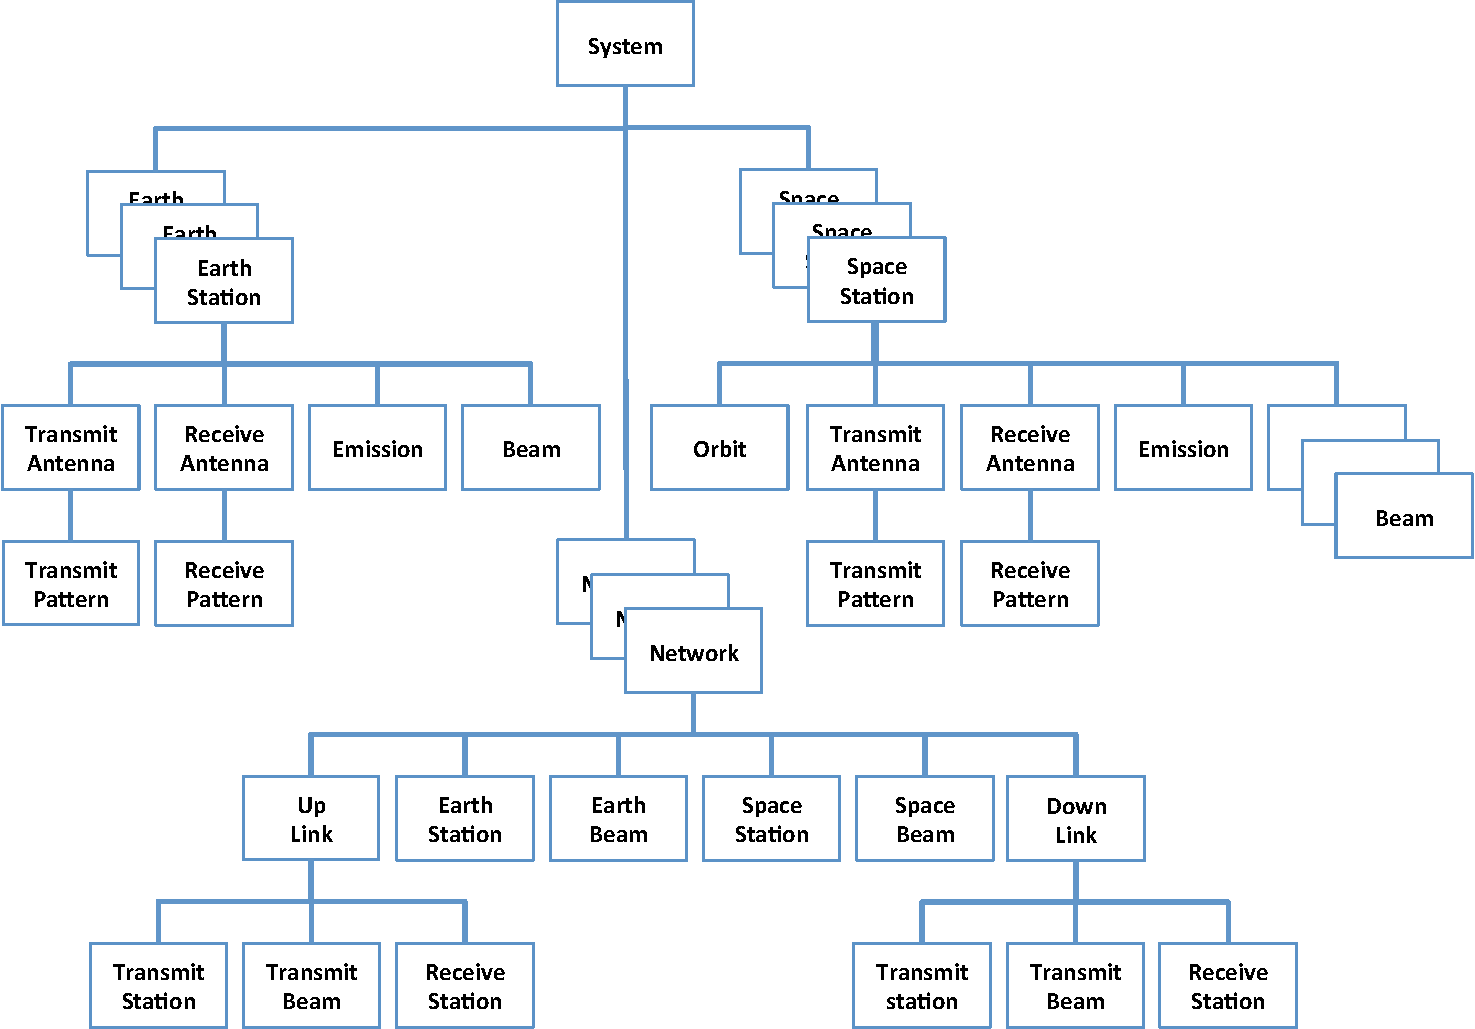
\includegraphics[width=7.0in]{figure-system-object-diagram.pdf}
    \end{center}
    \caption{System Object Diagram}\label{figure-system-object-diagram}
  \end{figure}
\end{landscape}

\subsection{Pattern Classes}

All reference antenna patterns published by the ITU are implemented in
the \texttt{\small pattern} package [F]. The reference antenna pattern
classes all inherit from parent class \texttt{\small Pattern}, and
depending on their purpose, from either \texttt{\small EarthPattern}
or \texttt{\small SpacePattern}, and from either or both of
\texttt{\small TransmitPattern} or \texttt{\small ReceivePattern}. A
typical \texttt{\small Pattern} is created as follows:
{\small
\begin{verbatim}
GainMax = 34;     % Maximum antenna gain [dB]
Efficiency = 0.7; % Antenna efficiency, fraction

pattern = PatternEREC013V01(GainMax, Efficiency);
\end{verbatim}
}
\noindent Note that the reference antenna pattern class constructors
do not all take the same arguments.

\subsection{Antenna Classes}

The antenna classes in the \texttt{\small antenna} package inherit
from parent class \texttt{\small Antenna}, and correspond to either
Earth or space stations. Although the functionality of the
\texttt{\small EarthStationAntenna} and \texttt{\small
  SpaceStationAntenna} class is largely identical, these classes
enforce correct use of the reference antenna patterns. With a
\texttt{\small Pattern} created as in the previous section, a typical
transmit \texttt{\small EarthStationAntenna} is created as follows:
{\small
\begin{verbatim}
name = 'NGSO ES Tx'; % Antenna name
gain = GainMax;      % Antenna gain
pattern_id = 1;      % Antenna pattern identifier

transmitAntenna = EarthStationAntenna(name, gain, pattern_id, pattern);
\end{verbatim}
}
and a receive \texttt{\small EarthStationAntenna} is created as
follows:
{\small
\begin{verbatim}
name = 'NGSO ES Rx'; % Antenna name
gain = GainMax;      % Antenna gain
pattern_id = 2;      % Antenna pattern identifier
noise_t = 150;       % Antenna noise temperature

receiveAntenna = EarthStationAntenna(name, gain, pattern_id, pattern, noise_t);
\end{verbatim}
}
\noindent Note that a receive antenna is created with the additional
argument \texttt{\small noise\_t}, and that the \texttt{\small gain},
\texttt{\small name} and \texttt{\small pattern\_id} properties are
descriptive only, and so can take any value without altering
functionality. As before, the reference antenna pattern class
constructors do not all take the same arguments.

\subsection{Emission Class}

The \texttt{\small Emission} class in the \texttt{\small station}
package contains parameters for describing the transmit waveform
characteristics. A Typical \texttt{\small Emission} is created as
follows:
{\small
\begin{verbatim}
design_emi = '1K20G1D--'; % Emission designator
pwr_ds_max = -60;         % Maximum power density
pwr_ds_min = NaN;         % Minimum power density
freq_mhz = 13000;         % Center frequency
c_to_n = NaN;             % Required C/N

emission = Emission( ...
  design_emi, pwr_ds_max, pwr_ds_min, freq_mhz, c_to_n);
\end{verbatim}
}
\noindent Note that the \texttt{\small design\_emi} property, which is
consistent with ITU filings, is descriptive only, and so can take any
value without altering functionality.

\subsection{Beam Class}

The \texttt{\small Beam} class in the \texttt{\small station} package
provides functionality for multiple beam assignment and beam
multiplexing. A typical \texttt{\small Beam} is created as follows:
{\small
\begin{verbatim}
name = 'IntLeoEarthSegment'; % Beam name
multiplicity = 1;            % Maximum number of divisions allowed
dutyCycle = 100;             % Duty cycle [%]

beam = Beam(name, multiplicity, dutyCycle);
\end{verbatim}
}
\noindent Note that the \texttt{\small name} property is descriptive
only, and so can take any value without altering functionality.

\subsection{Earth Station Class}

The \texttt{\small EarthStation} class in the \texttt{\small station}
package inherits from parent class \texttt{\small Station}, and
contains instances of a transmit and receive \texttt{\small Antenna},
an \texttt{\small Emission}, and a \texttt{\small Beam}. With
instances created as in the previous sections, an \texttt{\small
  EarthStation} is created as follows:
{\small
\begin{verbatim}
stationId      = 'wanted'; % Identifier for station
varphi         = 0;        % Geodetic latitude [rad]
lambda         = lla(2);   % Longitude [rad]
doMultiplexing = 0;        % Flag indicating whether to do multiplexing,
                           %   or not

earthStation = EarthStation(stationId, transmitAntenna, receiveAntenna, ...
                            emission, beam, varphi, lambda, doMultiplexing);
\end{verbatim}
}
\noindent Note that the \texttt{\small station\_id} property is
descriptive only, and so can take any value without altering
functionality.

\subsection{Orbit Classes}

The orbit classes in the \texttt{\small twobody} package inherit from
the parent classes \texttt{\small Orbit} and \texttt{\small
  TwoBodyOrbit}, and provide for the calculation of geocentric
equatorial inertial position using either Keplerian or equinoctial
orbital elements. A typical \texttt{\small KeplerianOrbit} is created
as follows:
{\small
\begin{verbatim}
a         = 1 + 1500 / EarthConstants.R_oplus; % Semi-major axis [er]
e         = 0.001;                             % Eccentricity [-]
i         = 80.0 * pi / 180;                   % Inclination [rad]
Omega     = 30.0 * pi / 180;                   % Right ascension of the
                                               %   ascending node [rad]
omega     = 60.0 * pi / 180;                   % Argument of perigee [rad]
M         = 130.0 * pi / 180;                  % Mean anomaly [rad]
epoch     = epoch_0;                           % Epoch date number
method    = 'halley';                          % Method to solve Kepler's equation:
                                               %   'newton' or 'halley'

orbit = KeplerianOrbit(a, e, i, Omega, omega, M, epoch, method);
\end{verbatim}
}

\subsection{Space Station Class}

The \texttt{\small SpaceStation} class in the \texttt{\small station}
package inherits from parent class \texttt{\small Station}, and
contains instances of a transmit and receive \texttt{\small Antenna},
an \texttt{\small Emission}, an array of \texttt{\small Beam}s, and an
\texttt{\small Orbit}. With instances created as in previous sections,
a typical \texttt{\small SpaceStation} is created as follows:
{\small
\begin{verbatim}
stationId = 'interfering'; % Identifier for station

spaceStation = SpaceStation( ...
  stationId, transmitAntenna, receiveAntenna, emission, beams, orbit);
\end{verbatim}
}
\noindent Note that the \texttt{\small station\_id} property is
descriptive only, and so can take any value without altering
functionality.

\subsection{System Class}

The \texttt{\small System} class in the \texttt{\small system} package
contains instances of \texttt{\small EarthStation}s, \texttt{\small
  SpaceStation}s, and \texttt{\small Network}s. However, the
\texttt{\small Network} instances are created during beam assignment,
rather than during creation of the \texttt{\small System}
instance. With instances created as in previous sections, a typical
\texttt{\small System} is created as follows:
{\small
\begin{verbatim}
losses = {}; % Propagation loss models to apply
dNm = datenum(2014, 10, 20, 19, 5, 0); % Current date number

system = System(earthStations, spaceStations, losses, dNm);
\end{verbatim}
}
\noindent Note that the \texttt{\small losses} property is descriptive
only, and so can take any value without altering functionality.

\subsection{Simulation}

Simulation of system performance involves assigning beams to create
networks, and computing link performance, possibly in the presence of
an interfering system, at each of a set of times which is sufficient
to represent the motion of the Earth and space stations. The
\texttt{\small Simulate} function in the \texttt{\small example}
package demonstrate the process of simulating the performance of a
wanted geostationary system consisting of a single space and Earth
station, in the presence of an interfering non-geostationary system
consisting of 18 Earth and 225 space stations in which the Earth
stations are located on a grid which includes the wanted Earth station
location. The typical order of calculations is as follows:
{\small
\begin{verbatim}
dNm_0 = datenum(2014, 10, 20, 19, 5, 0);
nSec = 1000;
parfor iDNm = [1 : nSec]
  dNm(iDNm) = dNm_0 + iDNm / 86400;
    
  if ~mod(iDNm, 4)
    interferingSystem.assignBeams([], [], dNm(iDNm));
      
  end % if
    
  performanceUp(iDNm) = wantedSystem.computeUpLinkPerformance( ...
      dNm(iDNm), interferingSystem, 1, 1, ref_bw);
  performanceDn(iDNm) = wantedSystem.computeUpLinkPerformance( ...
      dNm(iDNm), interferingSystem, 1, 1, ref_bw, 'DoIS', 1);
  performanceIS(iDNm) = wantedSystem.computeDownLinkPerformance( ...
      dNm(iDNm), interferingSystem, 1, 1, ref_bw);
   
end % for
\end{verbatim}
}

The following sections describe the engineering basis for the classes
required by this simulation procedure, again, in the order the classes
are created, in order to establish notation, and provide
references for additional information.

\section{Patterns, Antennas, Beams, and Emissions}

\subsection{Antenna Fundamentals}

As a radio wave arrives at an antenna, the antenna collects the power
contained in its effective aperture area, $A_e$.  For a perfect,
loss-less antenna, this effective aperture area would be equal to the
actual projected area, $A$.  In practice, the antenna will have some
losses, which are taken into account through the antenna efficiency,
$\eta$:
\begin{equation}
  A_e = \eta A
\end{equation}
where $A_e$ = effective aperture area (m$^2$), and $A$ = antenna area
($m^2$). Therefore, the effective area of a circular reflector can be
expressed as:
\begin{equation}
  A_e = \eta\pi r^2
\end{equation}
where $r$ = radius of antenna (m).

The relationship between the peak gain and effective area of an
antenna is given by:
\begin{equation}
  G = \frac{4\pi A_e}{\lambda^2}
\end{equation}
where $\lambda$ = wavelength (m). Note that the wavelength of the
electromagnetic wave is related to the frequency as follows:
\begin{equation}
  \lambda = \frac{c}{f}
\end{equation}
where $c$ = speed of light (299792458 m/s), and $f$ = frequency (Hz).
The off-axis gain of an antenna is typically expressed as a function
of the off-axis angle, $\Phi$, that is, $G(\Phi)$. Corresponding
reference antenna patterns published by the ITU are described in the
next section.

\subsection{Reference Antenna Patterns}

Figure \ref{figure-reference-antenna-pattern-equations} shows a
typical reference antenna pattern excerpted from Appendix 7 of the
Radio Regulations.
 
\begin{figure}
  \begin{center}
    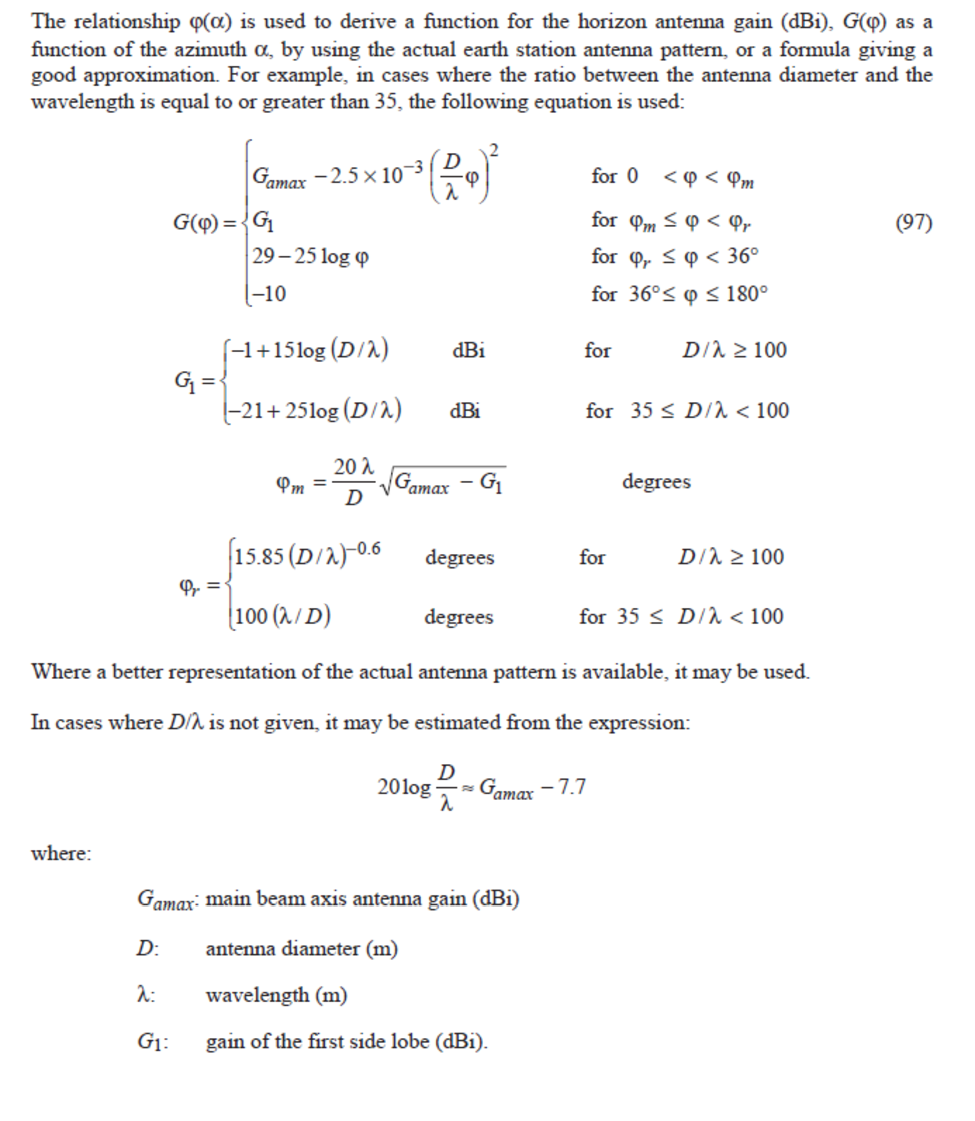
\includegraphics[width=5.0in]{figure-reference-antenna-pattern-equations.pdf}
  \end{center}
  \caption{Reference antenna pattern from Appendix 7}\label{figure-reference-antenna-pattern-equations}
\end{figure}

Reference patterns are defined by several regions: the main beam is the
area of highest gain near the pointing direction of the antenna, the
first side lobe region is represented by a constant gain value, the log
roll-off region is represented by the decreasing gain as a function of
off-axis angle, and the back lobe is represented by a constant value
for the far off-axis gain.  Figure
\ref{figure-reference-antenna-pattern-plot} shows the plot of a
typical reference antenna pattern and illustrates these four gain
regions.

\begin{figure}
  \begin{center}
    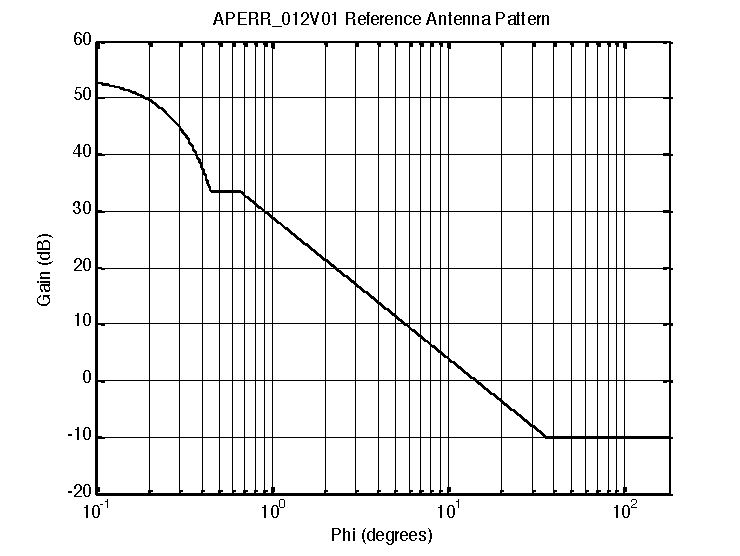
\includegraphics{figure-reference-antenna-pattern-plot.pdf}
  \end{center}
  \caption{Reference antenna pattern from Appendix 7}\label{figure-reference-antenna-pattern-plot}
\end{figure}

This example pattern from Appendix 7 requires the antenna peak gain
and the ratio of the antenna diameter to the wavelength ($D/\lambda$)
as input in order to calculate the gain at an off-axis angle.  Given
the frequency and antenna diameter, the antenna equations discussed
previously can be manipulated to derive the input parameters needed by
this Appendix 7 model:
\begin{eqnarray}
  A_e &=& \eta\pi\left(\frac{D}{2}\right)^2 \\
  G &=& \frac{4\pi A_e}{\lambda^2}
\end{eqnarray}
where $D$ = diameter of the antenna (m). Note that gain is typically
expressed in dB, in which case the gain is given by:
\begin{equation}
  G_{dB} = 10\log_{10}\frac{4\pi A_e}{\lambda^2}
\end{equation}
Given only the antenna gain (and efficiency, which can be assumed to
be $\approx$ 65\%), compute $D/\lambda$ from:
\begin{equation}
  G = \eta\left(\frac{\pi D}{\lambda}\right)^2
\end{equation}
or
\begin{equation}
  G_{dB} = 10\log_{10}\pi^2\eta + 20\log_{10}\left(\frac{D}{\lambda}\right)
\end{equation}
so
\begin{equation}
  \frac{D}{\lambda} = 10^{\frac{G_{dB} - 10\log_{10}\pi^2\eta}{20}}
\end{equation}
As an alternative, Appendix 7 provides an approximation of $D/\lambda$
based on the peak gain of the antenna:
\begin{equation}
  20\log_{10}(D/\lambda) \approx G_{dB} - 7.7
\end{equation}
So $D/\lambda$ can be approximated from:
\begin{equation}
  \frac{D}{\lambda} \approx 10^{\frac{G_{dB} - 7.7}{20}}
\end{equation}

This and the previous three subsections provide all of the objects
required to created a space or Earth station instance. The
following two sections describe the engineering basis for modeling
these stations, and for creating the corresponding classes.

\section{Space and Earth stations}

The space and Earth station classes in the \texttt{\small station} package
contain a transmit and receive antenna, an emission, and an array or
single beam, along with methods for computing position at a given
time.

\subsection{Space Stations}

Even though elaborate models have been developed to compute
the motion of artificial Earth satellites to high accuracy, the main
features of their orbits may still be described by a reasonably simple
approximation. [M\&G-2]

\subsubsection{Newton's Law of Gravitation}

A satellite is considered whose mass is negligible compared to the
Earth's mass $M_{\oplus}$. Assuming the Earth to be spherically
symmetric, the acceleration $\ddot{r}$ of the satellite is given by
Newton's law of gravity
\begin{equation}
  \ddot{\boldsymbol{r}} = -\frac{GM_{\oplus}}{r^2}\frac{\boldsymbol{r}}{r} \label{2.1}\tag{2.1}
\end{equation}
where $-\boldsymbol{r}/r$ denotes a unit vector pointing from the
satellite to the center of the Earth, which forms the origin of the
coordinate system.

$G$ is known with limited accuracy from torsion balance experiments
\begin{equation}
  G = (6.67259 \pm 0.00085)\cdot 10^{-11} \mathrm{m^3kg^{-1}s^{-2}} \label{2.2}\tag{2.2}
\end{equation}

$GM_{\oplus}$ is known with considerable accuracy from laser ranging
measurements of Earth satellites
\begin{equation}
  GM_{\oplus} = (398600.4405 \pm 0.001) \mathrm{km^3s^{-2}} \label{2.3}\tag{2.3}
\end{equation}

\subsubsection{The Two-Body Problem}

The study of the motion of a satellite in the spherically
symmetric $1/r^2$ force field of a central mass is usually referred to
as {\em Kepler's problem}, or as the {\em two-body} problem. [M\&G-2.1] It was
first solved in the second half of the 17th century by Isaac Newton.

\subsubsection{Plane Motion}

The fact that the force exerted on the satellite always
points to the Earth's center in the two-body problem has the immediate
consequence that the orbit is confined to a fixed plane for all
times. [M\&G-2.1.1] The satellite cannot leave the orbital plane, since the force
is always anti-parallel to the position vector and, therefore, does
not give rise to any acceleration perpendicular to the plane.

A mathematical description of this fact can be written as
\begin{equation}
  \boldsymbol{r}\times\dot{\boldsymbol{r}} = \boldsymbol{h}
                                           = \text{constant} \label{2.7}\tag{2.7}
\end{equation}
The vector $\boldsymbol{h}$ is the angular momentum per unit mass or
the specific angular momentum. It is related to the angular momentum
vector $\boldsymbol{l}$ by $\boldsymbol{l}=m\boldsymbol{h}$, where $m$
is the mass of the satellite.

\subsubsection{Law of Areas}

Equation \eqref{2.7} implies Kepler's second law, or the law of areas,
since
\begin{equation}
  \Delta A = \frac{1}{2}|\boldsymbol{r}\times\dot{\boldsymbol{r}}\Delta t| 
           = \frac{1}{2}|\boldsymbol{h}|\Delta t \label{2.8}\tag{2.8}
\end{equation}
is the area swept by the radius vector during the time $\Delta t$, and
since $h$ is a constant, the radius vector sweeps over equal areas in
equal time intervals.

\subsubsection{The Form of the Orbit}

Multiplying both sides of the equation of motion
\eqref{2.1} by $\boldsymbol{h}$, rearranging, using vector
multiplicative identities, and integrating yields
\begin{equation}
  \boldsymbol{h}\times\dot{\boldsymbol{r}}
  = -GM_{\oplus}\left(\frac{\boldsymbol{r}}{r}\right) - \boldsymbol{A} \label{2.12}\tag{2.12}
\end{equation}
where $\boldsymbol{A}$ is called the {\em Runge-Lenz} or {\em Laplace
  vector} (an additive constant of integration determined by the
initial position and velocity). [M\&G-2.1.2] Multiplying by $\boldsymbol{r}$, and
introducing $\nu$, the {\em true anomaly}, as the angle between
$\boldsymbol{A}$ and the position vector $\boldsymbol{r}$, $p$, the
{\em semi-latus rectum}, $p = h^2 / GM_{\oplus}$, and $e$, the {\em
  eccentricity}, $e = A / GM_{\oplus}$, yields
\begin{equation}
  r = \frac{p}{1 + e\cos\nu} \label{2.17}\tag{2.17}
\end{equation}
which is a conic section in polar coordinates describing an ellipse,
if $e < 1$, a parabola, if $e = 1$, or hyperbola, if $e > 1$. See
Fig. 2.2.

This discussion focuses on satellites in Earth orbit which exhibit an
elliptic orbit with $e < 1$.

\begin{figure}
  \begin{center}
    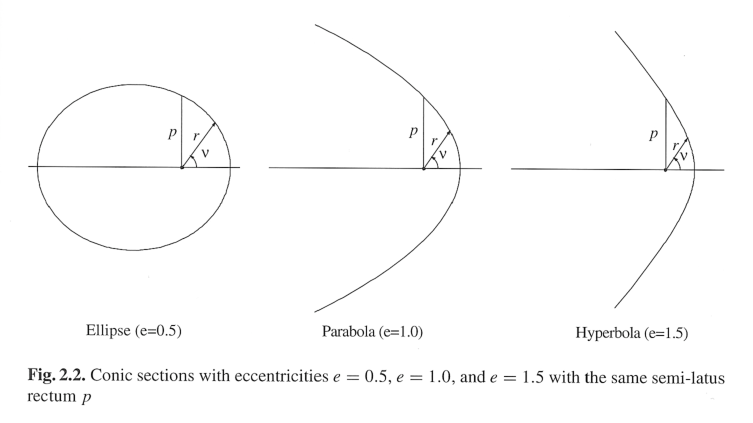
\includegraphics{figure-2-2.pdf}
  \end{center}
\end{figure}

\subsubsection{The Energy Integral}

Squaring both sides of \eqref{2.12} and simplifying yields
\begin{equation}
  v^2 = GM_{\oplus}\left(\frac{2}{r} - \frac{1}{a}\right) \label{2.22}\tag{2.22}
\end{equation}
which is called the {\em vis-viva law}. It is equivalent to the energy
statement that the sum of the kinetic energy, $(1/2)mv^2$, and the
potential energy, $-GmM_{\oplus}/r$, is constant during motion. [M\&G-2.1.3]

\subsubsection{Kepler's Equation}

\begin{figure}
  \begin{center}
    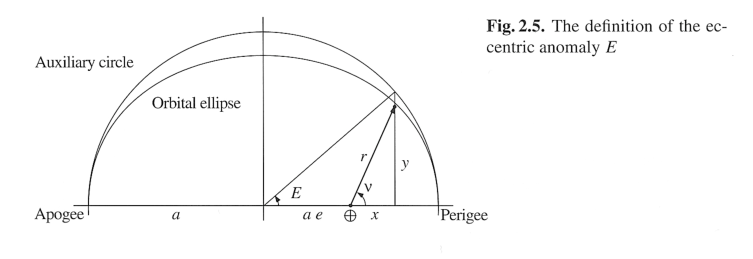
\includegraphics{figure-2-5.pdf}
  \end{center}
\end{figure}

Introduce the angle, $E$, between the center of a circle
circumscribing the orbit and the point of intersection of the orbit
and a line perpendicular to the line of apsides through the satellite
position, called the {\em eccentric anomaly}. [M\&G-2.2.1] See Fig. 2.5. Then
\begin{align}
  \hat{x} &= r\cos\nu =: a(\cos E - e) \notag \\
  \hat{y} &= r\sin\nu =: a\sqrt{1 - e^2}\sin E \label{2.30}\tag{2.30}
\end{align}
or equivalently
\begin{equation}
  r = a(1 - e\cos E) \label{2.31}\tag{2.31}
\end{equation}
Using these definitions, and the definition of the specific angular
momentum vector $h$, yields
\begin{equation}
  (1 - e\cos E)\dot{E} = n \label{2.34}\tag{2.34}
\end{equation}
where $n$, called the {\em mean motion}, is introduced to simply
notation and given by
\begin{equation}
  n = \sqrt{\frac{GM_{\oplus}}{a^3}} \label{2.35}\tag{2.35}
\end{equation}
Integrating with respect to time yields {\em Kepler's Equation}
\begin{equation}
  E(t) - e\sin E(t) = n(t - t_p) \label{2.36}\tag{2.36}
\end{equation}
where $t_p$ denotes the time of perigee passage. The right hand side
\begin{equation}
  M = n(t - t_p) \label{2.37}\tag{2.37}
\end{equation}
is called the {\em mean anomaly}. It changes by $360^{\circ}$ during
one revolution but -- in contrast to the true and eccentric anomalies
-- increases uniformly with time. The orbital period 
\begin{equation}
  T = \frac{2\pi}{n} \label{2.39}\tag{2.39}
\end{equation}

Kepler's equation can be solved by iterative methods
only. [M\&G-2.2.2] A common way is to start with an approximation of $E_0 = M$ or
$E_0 = \pi$ and employ Newton's method.

\subsubsection{The Orbit in Space}

\begin{figure}
  \begin{center}
    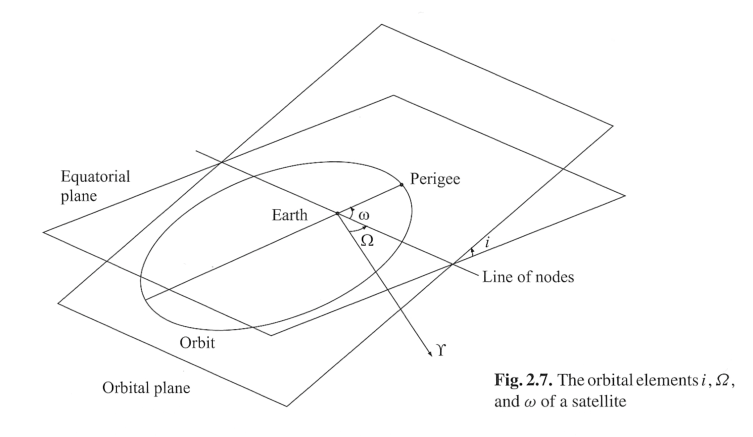
\includegraphics{figure-2-7.pdf}
  \end{center}
\end{figure}

Introduce the unit vector $\boldsymbol{P} =
\boldsymbol{A}/|\boldsymbol{A}|$, which points towards the perigee,
and the perpendicular unit vector $\boldsymbol{Q}$, corresponding to a
true anomaly of $\nu = 90^{\circ}$, to express the position by
\begin{equation}
  \boldsymbol{r}
  = \hat{x}\boldsymbol{P} + \hat{y}\boldsymbol{Q}
  = a(\cos E - e)\boldsymbol{P}
    + a\sqrt{1 - e^2}\sin E\boldsymbol{Q} \label{2.43}\tag{2.43}
\end{equation}
and the velocity by
\begin{equation}
  \dot{\boldsymbol{r}}
  = \dot{\hat{x}}\boldsymbol{P} + \dot{\hat{y}}\boldsymbol{Q}
  = \frac{\sqrt{GM_{\oplus}a}}{r}(-\sin E\boldsymbol{P}
    + \sqrt{1 - e^2}\cos E\boldsymbol{Q}) \label{2.44}\tag{2.44}
\end{equation}
See Fig 2.7. [M\&G-2.2.3]

\subsubsection{Two-line Element Sets}

A Two-Line Element (TLE) set is a data format encoding a list of
orbital elements of an Earth-orbiting object for a given point in
time, the epoch.  Using suitable prediction formula, the position and
velocity, together called the state, of the object at any point in the
past or future can be estimated.

The format uses two lines of 80-column ASCII text to store the data,
reflecting its origin in punch card format with one line per card.
The United States Air Force tracks objects in Earth orbit and creates
a corresponding TLE for each non-classified object, which is made
available on the Space-track website (https://www.space-track.org/).
A TLE may also include a title line that precedes the element data.
Figure \ref{figure-two-line-element-set-example} shows an example TLE
for the International Space Station. Figure
\ref{figure-two-line-element-set-decoding} shows how the data in a two
line element set is decoded.

\begin{table}
  \caption{Example two line element set}\label{figure-two-line-element-set-example}
  \small
\begin{verbatim}
ISS (ZARYA)
1 25544U 98067A   04236.56031392  .00020137  00000-0  16538-3 0  9993
2 25544  51.6335 344.7760 0007976 126.2523 325.9359 15.70406856328903
\end{verbatim}
\end{table}

\begin{landscape}
  \begin{figure}
    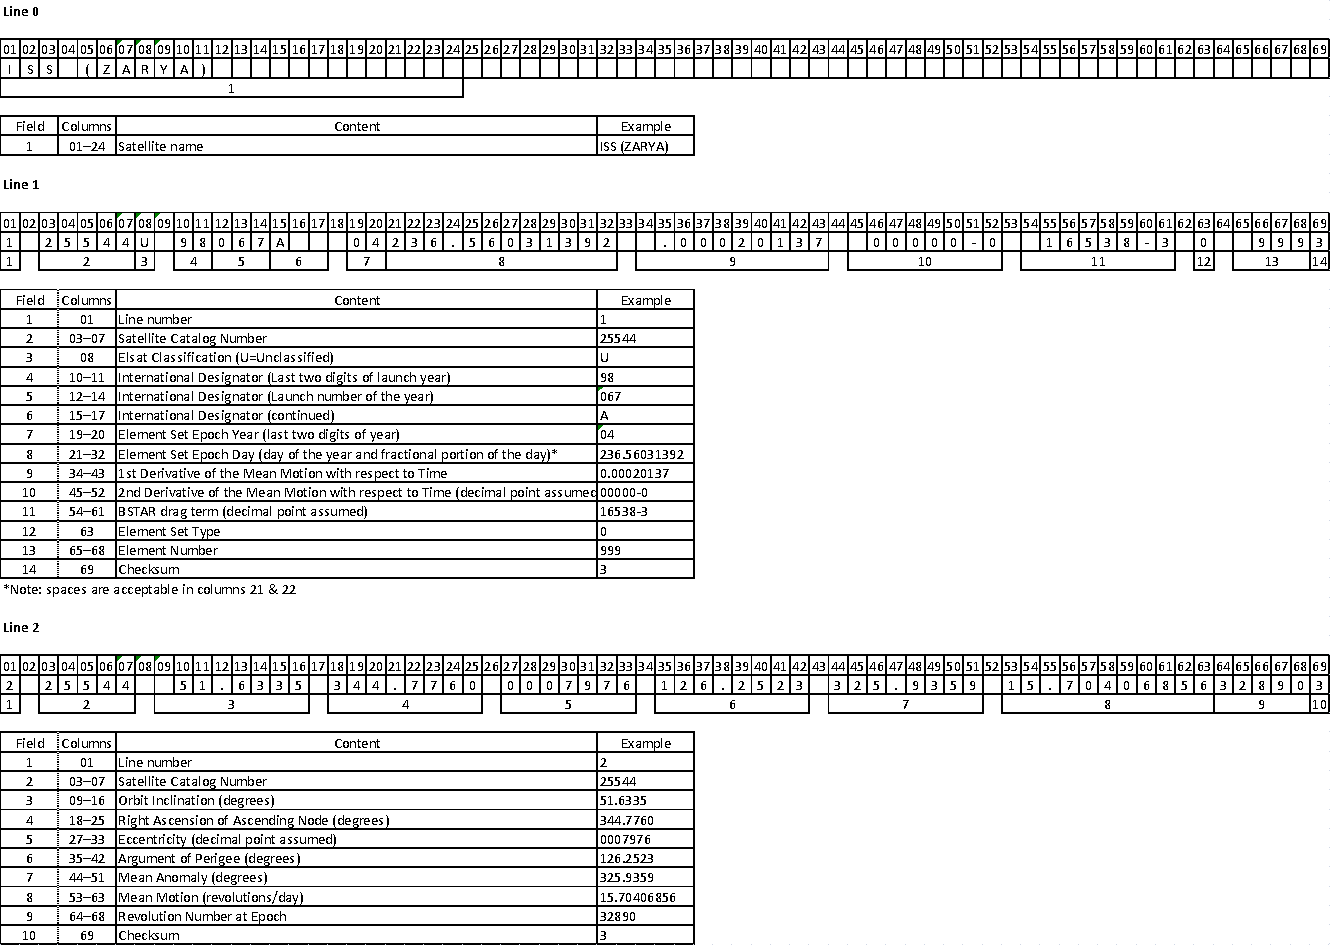
\includegraphics[width=7.0in]{figure-two-line-element-set-decoding.pdf}
    \caption{Two line element set decoding}\label{figure-two-line-element-set-decoding}
  \end{figure}
\end{landscape}

\subsubsection{The Equatorial Coordinate System}

The most common coordinate system for describing Earth-bound satellite
orbits is the geocentric {\em equatorial coordinate system}, which is
aligned with the Earth's rotation axis and equator. Its origin is the
center of the Earth, the $z$-axis points to the north pole and the
equatorial plane forms the $x$-$y$ reference plane. The $x$-axis is
aligned with the northern, {\em vernal equinox}, or the First Point of
Aries.

In order to describe the orientation of the orbital plane and the
perigee with respect to the equatorial coordinate system, three angles
are commonly employed
\begin{itemize}
\item[$i$] The {\em inclination} gives the angle of intersection
  between the orbital plane and the equator. An inclination of more
  than 90$^{\circ}$ means that the satellite's motion is retrograde,
  its direction of revolution around the Earth being opposite to that
  of the Earth's rotation.
\item[$\Omega$] The {\em right ascension of the ascending node}
  indicates the angle between the vernal equinox and the
  point on the orbit at with the satellite crosses the equator from
  south to north.
\item[$\omega$] The {\em argument of perigee} is the angle between the
  direction of the ascending node and the direction of the perigee.
\end{itemize}
See Fig 2.6.

\begin{figure}
  \begin{center}
    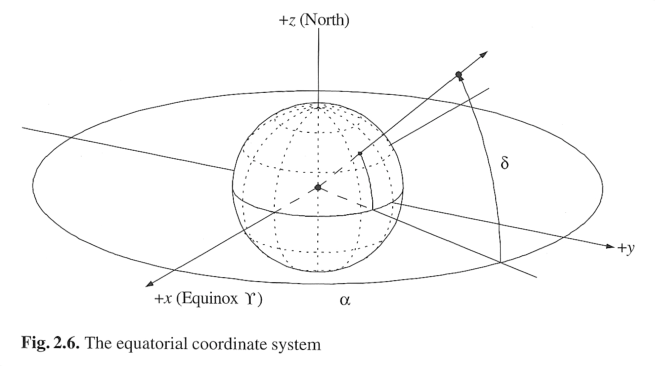
\includegraphics{figure-2-6.pdf}
  \end{center}
\end{figure}

In the orbital plane system, which is defined by the unit vectors
$\boldsymbol{P}$, $\boldsymbol{Q}$, $\boldsymbol{W} = \boldsymbol{h} /
h$, the coordinates are given by
\begin{equation}
  (\hat{x}, \hat{y}, \hat{z}) = (r\cos\nu, r\sin\nu, 0) \label{2.47}\tag{2.47}
\end{equation}
where
\begin{align}
  \boldsymbol{P} &= \left(
    \begin{array}{c}
      + \cos\omega\cos\Omega - \sin\omega\cos i\sin\Omega \\
      + \cos\omega\sin\Omega + \sin\omega\cos i\cos\Omega \\
      + \sin\omega\sin i
    \end{array}\right) \label{2.52}\tag{2.52} \\
  \boldsymbol{Q} &= \left(
    \begin{array}{c}
      - \sin\omega\cos\Omega - \cos\omega\cos i\sin\Omega \\
      - \sin\omega\sin\Omega + \cos\omega\cos i\cos\Omega \\
      + \cos\omega\sin i
    \end{array}\right) \label{2.53}\tag{2.53} \\
  \boldsymbol{W} &= \left(
    \begin{array}{c}
      + \sin i\sin\Omega \\
      - \sin i\cos\Omega \\
      + \cos i
    \end{array}\right) \label{2.54}\tag{2.54}
\end{align}
are referred to as {\em Gaussian vectors}.

In the equatorial system, the coordinates are given by
\begin{equation}
  \left(\begin{array}{c} x \\ y \\ z \end{array}\right)
  = \boldsymbol{R}_z(-\Omega)\boldsymbol{R}_x(-i)\boldsymbol{R}_z(-\omega)
  \left(\begin{array}{c} \cos\nu \\ \sin\nu \\ 0 \end{array}\right) \label{2.50}\tag{2.50}
\end{equation}
where
\begin{align}
  \boldsymbol{R}_x(\phi) &= \left(
    \begin{array}{ccc}
      1         & 0         & 0 \\
      0         & +\cos\phi & +\sin\phi \\
      0         & -\sin\phi & +\cos\phi
    \end{array}\right) \notag \\
  \boldsymbol{R}_y(\phi) &= \left(
    \begin{array}{ccc}
      +\cos\phi & 0         & -\sin\phi \\
      0         & 1         & 0 \\
      +\sin\phi & 0         & +\cos\phi
    \end{array}\right) \notag \\
  \boldsymbol{R}_z(\phi) &= \left(
    \begin{array}{ccc}
      +\cos\phi & +\sin\phi & 0 \\
      -\sin\phi & +\cos\phi & 0 \\
      0         & 0         & 1
    \end{array}\right) \label{2.55+}\tag{2.55+}
\end{align}
are rotation matrices about each coordinate axis.

\subsubsection{Force Model}

The inverse square law describes the gravitational
attraction of a point-like mass, and can always be shown to be true
for extended bodies, provided that they are built up of concentric
shells of constant density. [M\&G-3.1] Since this is a basic model of the
structure of the Earth, Keplerian orbits provide a reasonable first
approximation of satellite motion.

However, the trajectory of the satellite is not a closed
ellipse with an unchanging orientation in space, but an open curve
that continuously evolves with time, both in shape and
orientation. There are two types of orbit perturbations:
\begin{itemize}
\item The perturbations of gravitational origin which derive from a
  potential for which total energy is conserved, including the
  geopotential and the effects of the Sun and Moon, and
\item The non-gravitational perturbations that do not derive from a
  potential and that dissipate energy, including atmospheric drag and
  solar radiation pressure
\end{itemize}
Various perturbations of a satellite orbit are compared in Fig. 3.1.

\begin{figure}
  \begin{center}
    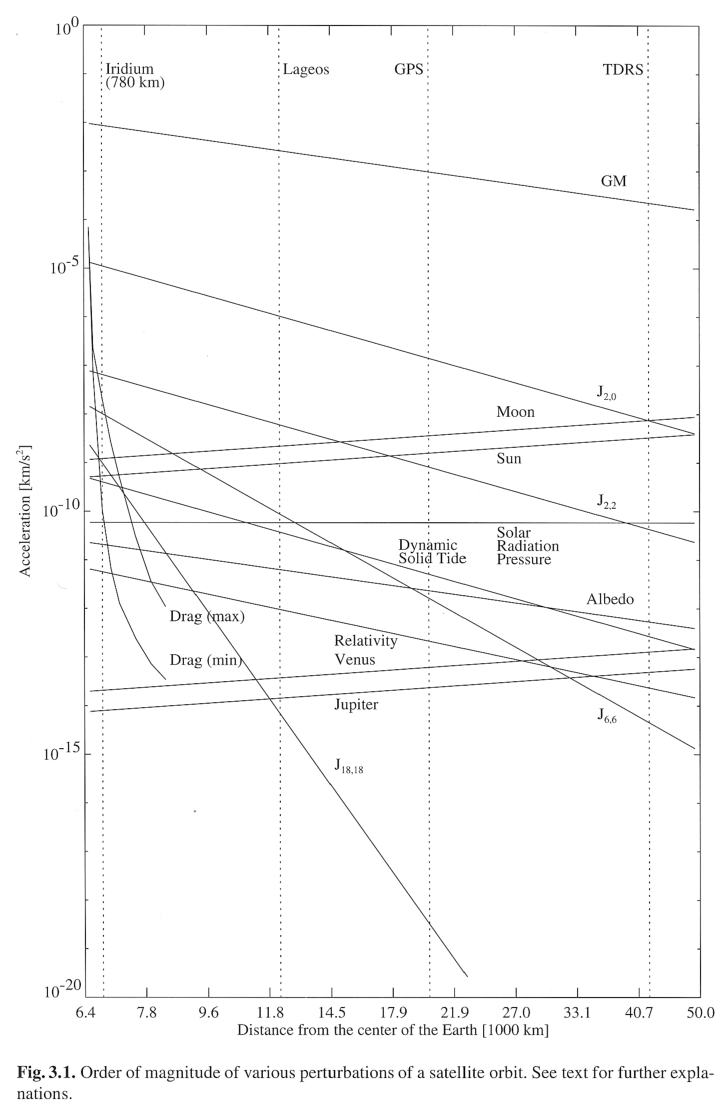
\includegraphics{figure-3-1.pdf}
  \end{center}
\end{figure}

\subsubsection{Geopotential}

Due to daily rotation, the Earth is not, however, a perfect
sphere, but has the form of an oblate spheroid with an equatorial
diameter that exceeds the polar diameter by about 20 km. [M\&G-3.1] The resulting
equatorial bulge exerts a force that pulls the satellite back to the
equatorial plane whenever it is above or below this plane and thus
tries to align the orbital plane with the equator. This perturbation
is about three orders of magnitude smaller than the central
attraction. Due to its angular momentum the orbit behaves like a
gyroscope, and reacts with a precessional motion of the orbital plane,
and a shift of the line of nodes by several degrees per day.

Assuming that the total mass of the Earth is concentrated
in the center of the coordinate system, the gravitational law
\begin{equation}
  \ddot{\boldsymbol{r}} = -\frac{GM_{\oplus}}{r^2}\frac{\boldsymbol{r}}{r} \label{2.1}\tag{2.1}
\end{equation}
can be used to calculate the acceleration of a satellite at
$\boldsymbol{r}$. [M\&G-3.2] For the following discussion of a more realistic
model, it is common to use an equivalent representation involving the
gradient of the corresponding gravity potential $U$
\begin{equation}
  \ddot{\boldsymbol{r}} = \nabla U \quad \text{with} \quad U
  = GM_{\oplus}\frac{1}{r} \label{3.3}\tag{3.3}
\end{equation}
This expression for the potential may be generalized to an arbitrary
mass distribution by summing up the contributions created by
individual mass elements $dm = \rho(\boldsymbol{s})d^3\boldsymbol{s}$
according to
\begin{equation}
  U = G \int
  \frac{\rho(\boldsymbol{s})d^3\boldsymbol{s}}
       {|\boldsymbol{r} - \boldsymbol{s}|} \label{3.4}\tag{3.4}
\end{equation}
where $\rho(\boldsymbol{s})$ is the density at point $\boldsymbol{s}$
inside the Earth, and $|\boldsymbol{r} - \boldsymbol{s}|$ is the
satellite's distance from $\boldsymbol{s}$.

\subsubsection{Expansion in Spherical Harmonics}

In order to evaluate the integral in the above equation,
the inverse of the distance may be expanded in a series of Legendre
polynomials. [M\&G-3.2.1] For $r > s$, which holds for all points $\boldsymbol{r}$
outside a circumscribing sphere, one has
\begin{equation}
  \frac{1}{|\boldsymbol{r} - \boldsymbol{s}|}
  = \frac{1}{r}\sum_{n = 0}^{\infty}\left(\frac{s}{r}\right)^nP_n(\cos\gamma)
  \quad \text{with} \quad \cos\gamma = \frac{\boldsymbol{r}\cdot\boldsymbol{s}}{rs}
  \label{3.5}\tag{3.5}
\end{equation}
Here
\begin{equation}
  P_n(u) = \frac{1}{2^nn!}\frac{d^n}{du^n}(u^2 - 1)^n \label{3.6}\tag{3.6}
\end{equation}
is the Legendre polynomial of degree $n$, and $\gamma$ is the angle
between $\boldsymbol{r}$ and $\boldsymbol{s}$.

By introducing the longitude $\lambda$ (positive towards the East) and
the geocentric latitude $\phi$ of the point $\boldsymbol{r}$ according
to
\begin{align}
  x &= r\cos\phi\cos\lambda \nonumber \\
  y &= r\cos\phi\sin\lambda \nonumber \\
  z &= r\sin\phi \label{3.7}\tag{3.7}
\end{align}
as well as the corresponding quantities $\lambda'$ and $\phi'$ for
$\boldsymbol{s}$, one can make use of the addition theorem of Legendre
polynomials, which states that
\begin{equation}
  P_n(\cos\gamma) = \sum_{m = 0}^n(2 - \delta_{0m}
  \frac{(n - m)!}{(n + m)!}P_{nm}(\sin\phi)P_{nm}(\sin\phi')\cos(m(\lambda - \lambda'))
  \label{3.8}\tag{3.8}
\end{equation}
where $P_{nm}$ (the associated Legendre polynomial of degree $n$ and
order $m$) is defined as
\begin{equation}
  P_{nm} = (1 - u^2)^{m/2}\frac{d^m}{du^m}P_n(u) \label{3.9}\tag{3.9}
\end{equation}

One is now able to write the Earth's gravity potential in the form
\begin{equation}
  U = \frac{GM_{\oplus}}{r}\sum_{n = 0}^{\infty}\sum_{m = 0}^n
  \frac{R_{\oplus}^n}{r^n}P_{nm}(\sin\phi)(C_{nm}\cos(m\lambda)
  + S_{nm}\sin(m\lambda)) \label{3.10}\tag{3.10}
\end{equation}
with coefficients
\begin{align}
  C_{nm} &= \frac{2 - \delta_{0m}}{M_{\oplus}}\frac{(n - m)!}{(n + m)!}
  \int\frac{s^n}{R_{\oplus}^n}P_{nm}(\sin\phi')
  \cos(m\lambda')\rho(\boldsymbol{s})d^3\boldsymbol{s} \nonumber \\
  S_{nm} &= \frac{2 - \delta_{0m}}{M_{\oplus}}\frac{(n - m)!}{(n + m)!}
  \int\frac{s^n}{R_{\oplus}^n}P_{nm}(\sin\phi')
  \sin(m\lambda')\rho(\boldsymbol{s})d^3\boldsymbol{s} \label{3.11}\tag{3.11}
\end{align}
which describe the dependence of $U$ on the Earth's internal mass
distribution. Geopotential coefficients with $m = 0$ are called {\em
  zonal} coefficients, since they describe the potential that does not
depend on the longitude. All $S_{n0}$ vanish due to their definition,
and the notation
\begin{equation}
  J_n = -C_{n0} \label{3.12}\tag{3.12}
\end{equation}
is commonly used for the remaining zonal terms. The other geopotential
coefficients are known as {\em tesseral} and {\em sectorial}
coefficients for ($m < n$) and ($m = n$), respectively. See Table 1.

\begin{table}
  \caption{Geopotential coefficients up to degree and order three [M\&G-Table-3.2]}
  \begin{center}
    \begin{tabular}{|c|cccc|}
      \hline
      $C_{nm}$ & $m = 0$ & 1 & 2 & 3 \\
      \hline
      $n = 0$ & + 1.00 & & & \\
      1 & 0.00 & 0.00 & & \\
      2 & $-1.08\cdot 10^{-3}$ & 0.00 & $+1.57\cdot 10^{-6}$ & \\
      3 & $+2.53\cdot 10^{-6}$ & $+2.18\cdot 10^{-6}$ & $+3.11\cdot 10^{-7}$ & $+1.02\cdot 10^{-7}$ \\
      \hline
      $S_{nm}$ & $m = 0$ & 1 & 2 & 3 \\
      \hline
      $n = 0$ & 0.00 & & & \\
      1 & 0.00 & 0.00 & & \\
      2 & 0.00 & 0.00 & $-9.03\cdot 10^{-7}$ & \\
      3 & 0.00 & $+2.68\cdot 10^{-7}$ & $-2.12\cdot 10^{-7}$ & $+1.98\cdot 10^{-7}$ \\
      \hline
    \end{tabular}
  \end{center}
\end{table}

Because the internal mass distribution of the Earth is
not known, the geopotential coefficients cannot be calculated from the
defining equation, but have to be determined indirectly using
satellite tracking, surface gravimetry, and satellite altimeter
data. [M\&G-3.2.3] Various government and research organization undertake to
develop these models. For example, a cooperation between the National
Aeronautics and Space Administration (NASA) Goddard Space Flight
Center (GSFC), the University of Texas Center for Space Research
(CSR), the Centre National d'\'{E}tudes Spatiales (CNES) led to the
Joint Gravity Model (JGM) series, with JGM-3 being published in 1996.

\subsubsection{Secular Perturbations}

First-order secular variations of the classical elements
affect the right ascension of the ascending node, the argument of
perigee, and the mean motion, or, equivalently, the initial value of
the mean anomaly, to produce a linear change with time given by:
\begin{eqnarray}
  \dot{\Omega} &=& -\frac{3nJ_2}{2p^2}\cos(i) \\
  \dot{\omega} &=& \frac{3nJ_2}{4p^2}(4 - 5\sin^2(i)) \\
  \dot{M_0} &=& \frac{3nJ_2(1 - e^2)}{4p^2}(2 - 3\sin^2(i))
\end{eqnarray}
where the semi-latus rectum $p = a * (1 - e^2)$ with semi-major axis
$a$ expressed in Earth radii. [V-9.6.1]

\subsection{Earth Stations}

\subsubsection{Earth Rotation}

The rotation of the Earth is represented by the right ascension, in
degrees, of the Greenwich meridian as a function of time given by
\begin{equation}
  \Theta = 280.4606 + 360.9856473d
\end{equation}
where $d$ is the time in days since noon on January 1, 2000.

\subsubsection{Geodetic Datums}

The World Geodetic System 1972 (WGS1972) and 1984 (WGS1984)
have been established by the United States Department of Defense (DoD)
and the Defense Mapping Agency (DMA) for use with the TRANSIT and GPS
satellite navigation systems. [M\&G-5.5]

Unlike the geocentric latitude $\phi'$ that specifies the inclination
of the position vector with respect to the equatorial plane, the
geodetic latitude $\phi$ gives the angle between the Earth's equator
and the normal to the reference ellipsoid, or the elevation of the
North Celestial Pole about the local tangent plane. See Fig. 5.12.

The relation between Cartesian and geodetic coordinates is give by
\begin{equation}
  \boldsymbol{r} = \left(\begin{array}{c}
    (N + h)\cos\varphi\cos\lambda \\
    (N + h)\cos\varphi\sin\lambda \\
    ((1 - f)^2N + h)\sin\phi
  \end{array}\right) \label{5.83}\tag{5.83}
\end{equation}
where
\begin{equation}
  N = \frac{R_{\oplus}}{\sqrt{1 - f(2 - f)\sin^2\varphi}} \label{5.84}\tag{5.84}
\end{equation}
For WGS84 $R_{\oplus} = 6,378,137$ m and $1/f = 298.257223563$.

\begin{figure}
  \begin{center}
    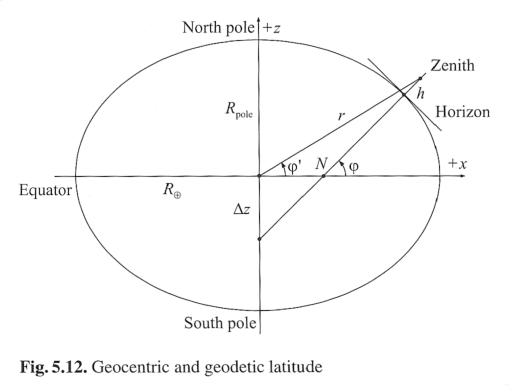
\includegraphics{figure-5-12.pdf}
  \end{center}
\end{figure}

\section{Link Performance}

The basic equation of a link relates the received carrier power to the
noise level of the receive system, which is the carrier-to-noise
ratio, $C/N$.  In the clear sky condition (i.e., no additional
propagation losses due to precipitation), the $C/N$ is given by:
\begin{eqnarray}
  C / N_{UP} &=& PD_{ES,W} + G_{ES,W}(\theta_W) \nonumber \\
  && - SL + G_{SS,W}(0) - 10\log_{10}(T) - k \\
  C / N_{DN} &=& PD_{SS,W} + G_{SS,W}(0) \nonumber \\
  && - SL + G_{ES,W}(\theta_W) - 10\log_{10}(T) - k
\end{eqnarray}
where subscript $X$ refers to link direction, $C/N_{X}$ = link
carrier-to-noise ratio (dB), $PD_{ES,W}$ = power density of earth
station wanted signal (dBW/Hz), $PD_{SS,W}$ = power density of space
station wanted signal (dBW/Hz), $G_{ES,W}(\theta_W)$ = co-pol gain of
wanted earth station in direction of wanted space station (dBi), $SL$
= space loss (dB), $G_{SS,W}$ = gain of wanted space station in
direction of wanted earth station (dBi), $T$ = receive noise
temperature (K), and $k$ = Boltzman’s constant (-228.6 dBW/Hz-K).

The carrier-to-noise ratio is just the transmit power less the
propagation loss plus the receive gain compared to receiver thermal
noise.  If the C/N of the link exceeds the required level, the link is
said to have positive link margin.  Links with positive margin have
sufficient power to transmit information at the desired rate and
accuracy, and the link is said to be closed.  Negative margin means
the link does not close since it has insufficient power to meet the
performance requirements.

The carrier-to-interference ratio (C/I) is calculated from the
following equations:
\begin{eqnarray}
  C_{DN} &=& PD_{SS,W} + G_{SS,W}(0) - SL + G_{ES,W}(\theta_W) \\
  C_{UP} &=& PD_{ES,W} + G_{ES,W}(\theta_W) - SL + G_{SS,W}(0) \\
  I_{DN} &=& PD_{SS,I} + G_{SS,I}(0) - SL + G_{ES,W}(\theta_I) \\
  I_{UP} &=& PD_{ES,I} + G_{ES,I}(\theta_I) - SL + G_{SS,W}(0)
\end{eqnarray}
where subscript $X$ refers to link direction, $C_X$ = link carrier
power density (dBW/Hz), $I_{X}$ = co-pol interference power density
(dBW/Hz), $PD_{ES,I}$ = power density of earth station interfering
signal (dBW/Hz), $PD_{SS,I}$ = power density of space station
interfering signal (dBW/Hz), $G_{SS,I}$ = gain of interfering space
station in direction of wanted earth station (dBi),
$G_{ES,W}(\theta_I)$ = co-pol gain of wanted earth station in
direction of interfering space station (dBi), $G_{ES,I}(\theta_I)$ =
co-pol gain of interfering earth station in direction of wanted space
station (dBi) and
\begin{equation}
  C / I_X = C_X - I_X + FDR + PD
\end{equation}
with parameters expressed in dB, and
\begin{equation}
  C / (N + I)_X = 10\log_{10}\left(\left(\frac{C}{(N + I)_X}\right)\times FDR \times PD\right)
\end{equation}
with parameters expressed as power ratios, where $FDR$ = frequency
dependent rejection (dB, assumed 0 for this analysis), and $PD$ =
polarization discrimination (dB). Note that polarization
discrimination ($PD$) is derived from the group polarization symbol
given in the ITU filing data. Using the $C/I$ ratio, the total
$C/(N+I)$ and availability both with and without interference are
calculated assuming the rain fade statistics given by Recommendation
ITU-R P.618-9.

\subsection{Noise Temperature and Figure of Merit}

Noise power at the receiver input is due both to the internal sources
such as the inherent movement of electrons, and external sources such
as contribution from the antenna.  The noise power, $N$, or noise
spectral density, $N_0$, is related to the noise temperature, $T$, as
follows:
\begin{eqnarray}
  N &=& kTB \\
  N_0 &=& kT
\end{eqnarray}
where $N$ = Noise power (W), $N_0$ = Noise spectral density (W/Hz),
$T$ = Noise temperature (K), $B$ = Noise bandwidth (Hz), and $k$ =
Boltzmann’s constant (1.38065×10-23 J/K).

In calculating link budgets the noise spectral density or the noise
temperature is often used instead of the total noise power so that
there is no need to specify the bandwidth in which the noise is
measured.

The noise caused by a receiver is usually expressed in terms of an
equivalent amplifier noise temperature $T_R$, which is defined as the
temperature of a noise source that, when connected to the input of a
noiseless receiver, gives the same noise at the output as the actual
receiver.

\subsection{Free Space Loss}

The free-space propagation loss in dB is given by:
\begin{equation}
  FSL = 20\log_{10}\left(\frac{4\pi d}{\lambda}\right)
\end{equation}
where $d$ = distance between space station and earth station (m), and
$\lambda$ = wavelength (m).

\section{References}

\begin{description}
\item[F] Filipova, T., \emph{Antenna Patterns Reference Manual},
  International Telecommunication Union, 2007.
\item[M\&G] Montenbruck, O., Gill, E., \emph{Satellite Orbits, Models,
  Methods, Applications}, Springer-Verlag, 2001.
\item[V] Vallado, D. A., \emph{Fundamentals of Astrodynamics and
  Applications, Second Edition}, Microcosm Press and Kluwer Academic
  Publishers, 2004.
\end{description}

\end{document}
